% 3 - Technical Description. Here you explain the technical work you have carried out.
% You may include code snippets where relevant, and refer to source code in the project files.
% Try to explain the development choices you did taking into account important properties such as deployability, availability, reusability, security, modifiability, performance.

\section{Technical Description}\label{sec:technicalDescription}
In this section the technicalities of the project is explained.
First the spec will explained and then every aspect into more detail.
A flowchart of the stack can be seen below:\\
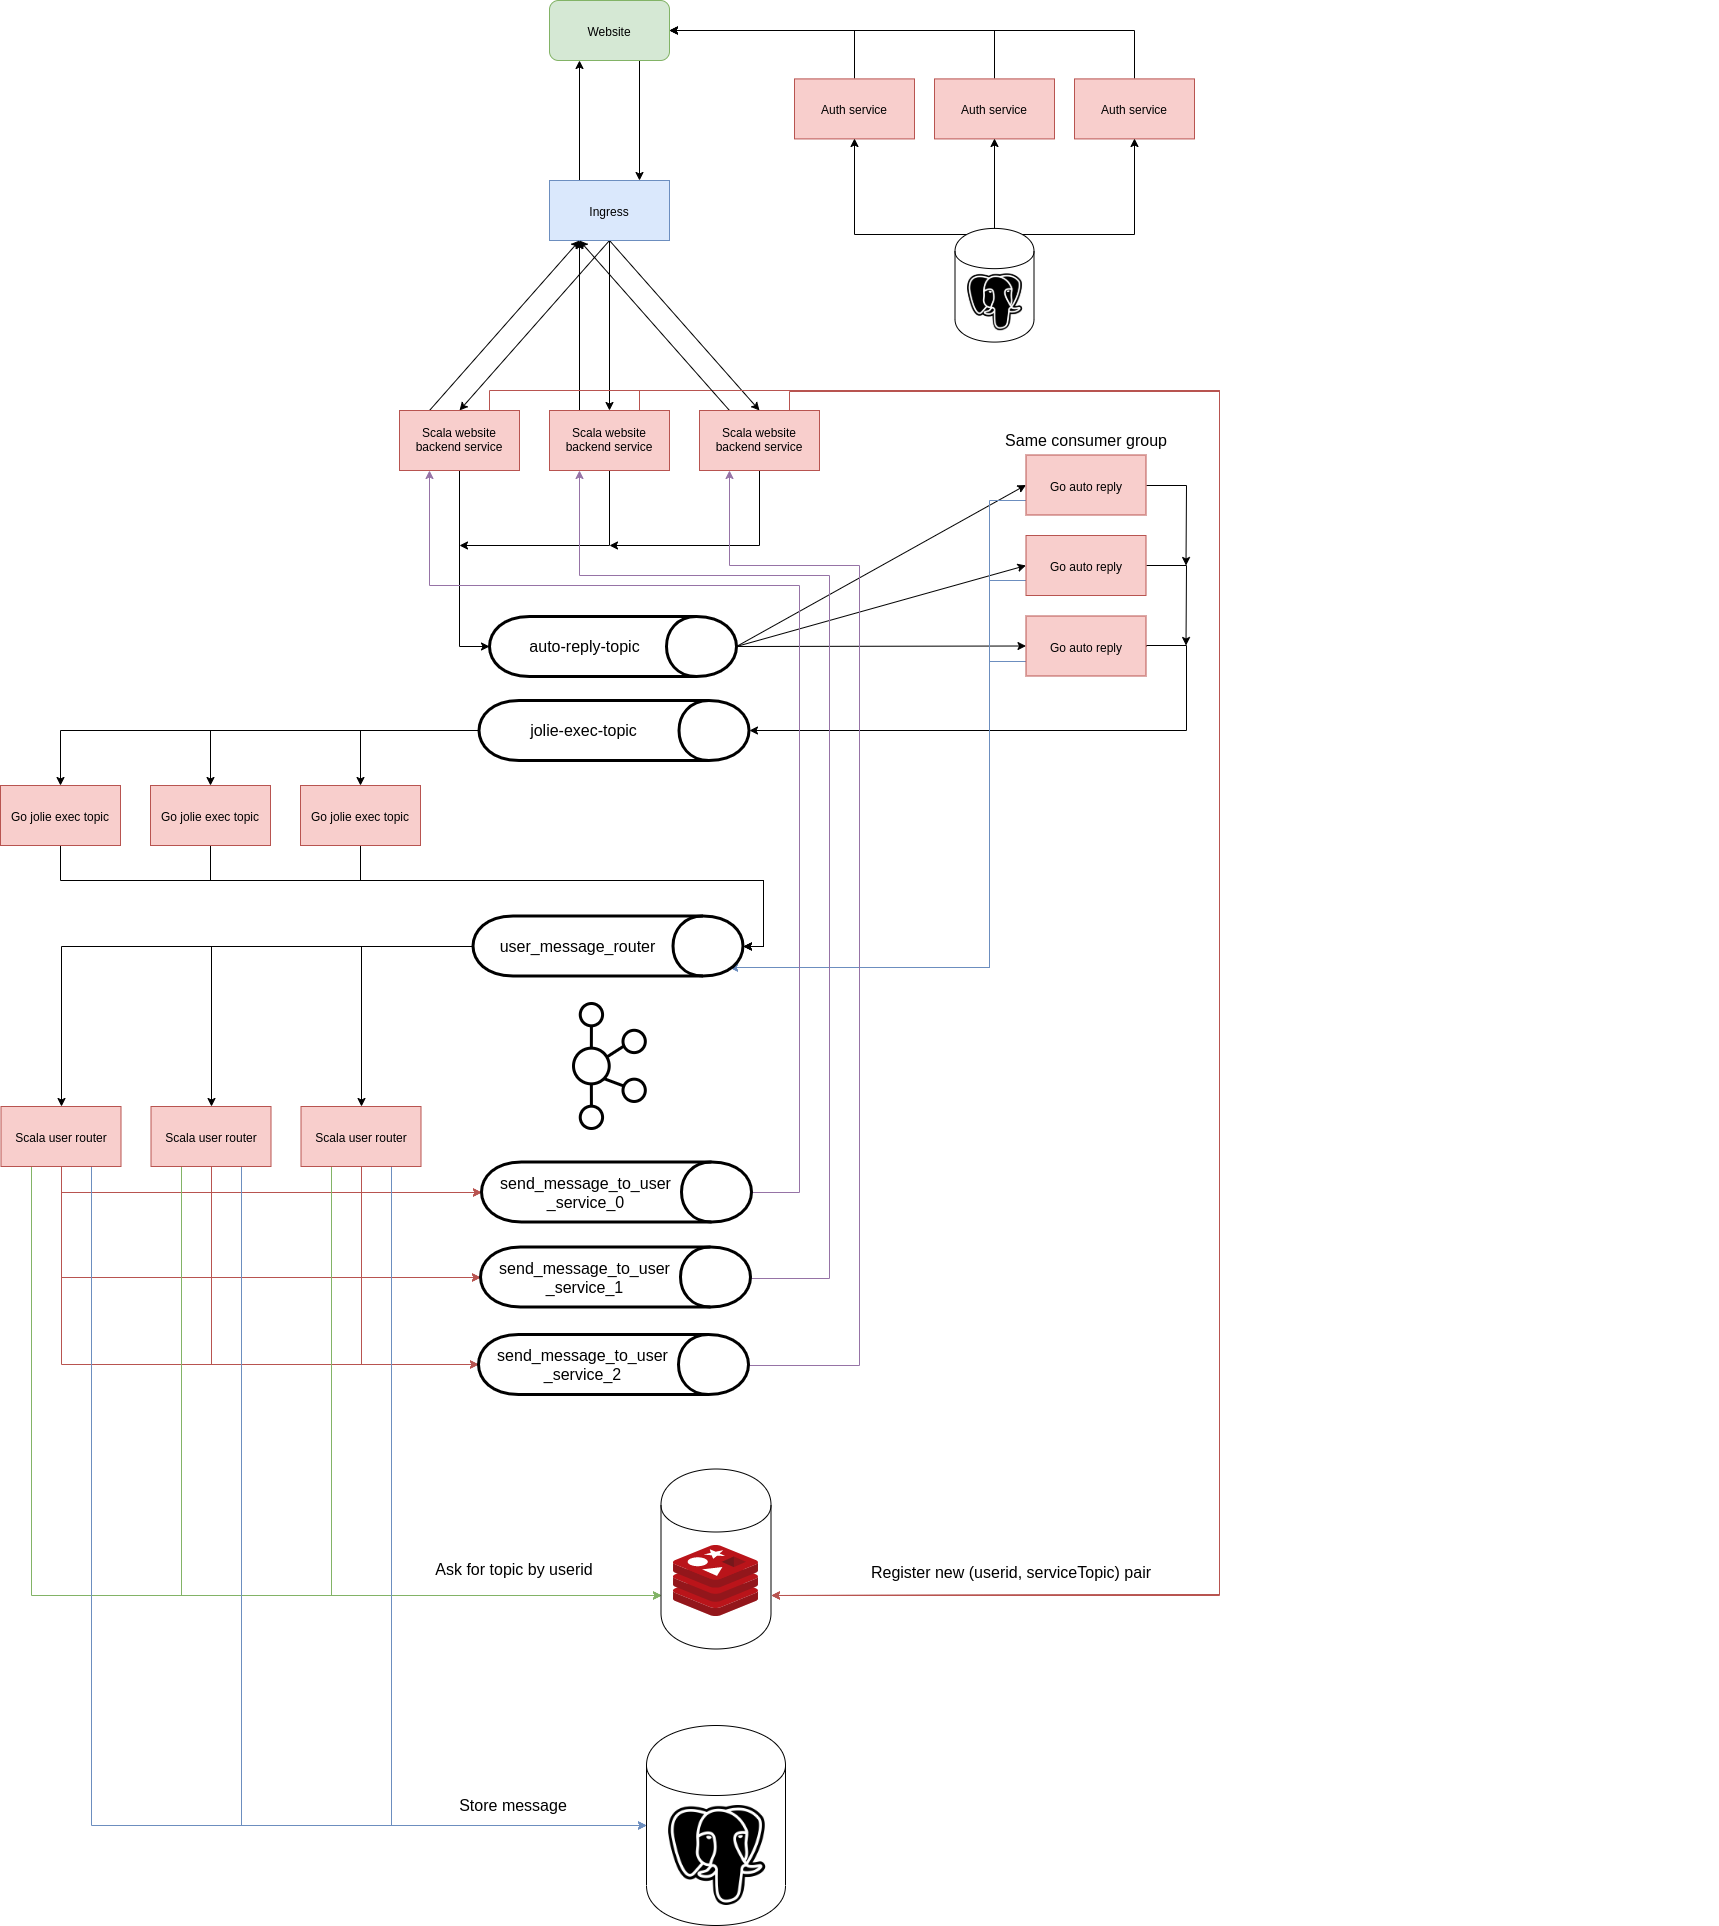
\includegraphics[scale=0.38]{stack.png}
\\
In the spec we use an event sourcing like technique.
This includes a stateful data-structure that every service knows the structure of.
This structure contains any data about a message that a service would need to know, as well as the sender user.\\
\begin{lstlisting}
    {
        "messageUid": "c0a630d2-8db3-4a03-9e19-7141582f37aa",
        "sessionUid": "cf2bd7ca-ba13-40d9-8fb7-bab2064028d4",
        "messageBody": "Hello, world!",
        "senderId": 42,
        "recipientIds": [12, 8],
        "fromAutoReply": false,
        "eventDestinations": ["TOPIC1", "TOPIC2"]
    }
\end{lstlisting}
\begin{enumerate}
    \item \texttt{messageUid} a UUID that represents the message id.
    \item \texttt{sessionUid} a UUID to represent the user session (websocket session).
    \item \texttt{messageBody} this is the full message.
    \item \texttt{senderId} this is the user id of the sender.
    \item \texttt{recipientIds} these id's represent the recipient user id's.
    \item \texttt{fromAutoReply} this represents if the message was generated through pragmatic methods.
    \item \texttt{eventDestinations} this represents the topics (services) that the message must go through, usually a message ends in the router.
\end{enumerate}

\subsection{Microservices}
\subsubsection{Webserver (website backend)}
This service has 5 simple but important objectives.
\begin{enumerate}
    \item To serve the static single page React application.
    \item To handle user websockets through the kubernetes ingress \& insert itself as the manager of a user websocket.
    \item To check authentication when a user makes a request.
    \item To "bootstrap" a message, by inserting into one of these event sourcing models (see the JSON structure in above).
    \item To route messages back to the recipient user websockets.
\end{enumerate}
The service is written in scala and is independently scalable, has no state, storage or any stateful requirements.
It is fault tolerant and secure through JWT using HMAC256 symmetric private key encryption.
\subsubsection{Auto reply}
\subsubsection{Jolie exec}
\subsubsection{Router}
The router service is responsible for routing messages to the correct services, eg the one managing the websocket for the recipient user.
The router service simply makes a lookup in redis for the key of the self-registered managed websocket, and sends the message to the found web-servers.
% static services
\subsection{Static services}
\subsection{Deployability}
\subsection{Reusability}
\subsection{Performance}
\subsection{Fault tolerance}